



\documentclass[dvipsnames,hyperref={pdfpagelabels=false}]{beamer}
% beamer already loads hyperref; do NOT load \usepackage{hyperref} again.
\usepackage{listings}
\usepackage{lmodern}
\usepackage{fontspec}
\usepackage{xeCJK}
\setCJKmainfont{Noto Sans CJK TC}
\setCJKsansfont{Noto Sans CJK TC}
\setCJKmonofont{Noto Sans Mono CJK TC}
\usepackage[english]{babel}
\usepackage{amsmath,amssymb,amsfonts,amsthm}

% hyperref settings (since beamer already loads hyperref)
\hypersetup{
  colorlinks=true,
  urlcolor=blue,
  citecolor=blue,
  pdfborder={0 0 0}
}

\usepackage{booktabs}
\usepackage{colortbl}
\usepackage{xcolor}

\usepackage{accsupp}% http://ctan.org/pkg/accsupp
\newcommand{\emptyaccsupp}[1]{\BeginAccSupp{ActualText={}}#1\EndAccSupp{}}


\usepackage{tikz}
\usetikzlibrary{arrows,decorations.pathmorphing,backgrounds,fit,positioning,shapes.symbols,chains}
\usetikzlibrary{tikzmark}
\usepackage{threeparttable}
\newcommand{\indep}{\perp\!\!\!\perp}
\newcommand{\nindep}{\not\!\perp\!\!\!\perp}

\beamertemplatefootpagenumber

\usepackage{listings}
%%%%%%%%%%%%%%%%%%%%%%%%%%%%%%%%%%%%%%%%%%%%%%%%%%%%%%%%%%%%%%%%%%%%%%%%%%%%%%
% LaTeX snippet: language and style definition of Stata for listings package.
%                [listings](http://www.ctan.org/pkg/listings) 
%                [Stata](http://www.stata.com/)
%
% Usage:
%     Copy the code into your preamble, or import it by `\include` .
%     then in your doc:
%     \lstinputlisting[style=numbers]{DO-SCRIPT}
%     \lstinputlisting[style=numbers, style=stata-editor]{DO-SCRIPT}
%     \lstinputlisting[style=nonumbers, frame=none]{DO-SCRIPT}
% How it works:
%     - The language is defined by `\lstdefinelanguage{Stata}`
%     - Four styles is defined by `\lstdefinestyle{STYLE-NAME}`, 
%       they are: numbers and no numbers, plain(black and white) and colorful
%       (colored roughly like stata editor.)
% Tips:
%     - Generally you only need to set your default in the last part,
%       that is, code inside of `\lstset`.
%     - Add more keywords(I can not list all of them) in the `\lstset` part.
%     - Do NOT leave any blank lines in commands
%       (`\lstddefinelanguage', `\lstdefinestyle` and `\lstset`)
%
% update: 2014-04-16
% version: 0.1
% author: kongs
% licence: MIT
% url: https://gist.github.com/kongs-sublime/10862838
%
% TODO: 
%       - finish keyword list.
%       - precise colors that match stata editor?
%       - make it flexible(fonts and style)
%
%%%%%%%%%%%%%%%%%%%%%%%%%%%%%%%%%%%%%%%%%%%%%%%%%%%%%%%%%%%%%%%%%%%%%%%%%%%%%%


% langugae defination
\lstdefinelanguage{Stata}{
	% Left for users to add missing commands,
	% with possibility of choosing different style.
	morekeywords=,
	% Popular add-on commands
	morekeywords=[2]{cntrade, chinafin, 
		wbopendata, spmap,
	},
	% System commands
	morekeywords=[3]{regress, summarize, 
		display,
	},
	% Keywords
	morekeywords=[4]{forvalues, if, foreach, set},
	% Built-in functions
	morekeywords=[5]{rnormal, runiform},
	morecomment=[l]{//},
	% morecomment=[l]{*},  // `*` maybe used as multiply operator. So use `//` as line comment.
	morecomment=[s]{/*}{*/},
	% morecomment=[s]{,}{//},
	% The following is used by macros, like `lags'.
	morecomment=[n][keywordstyle9]{`}{'},
	morestring=[b]",
	sensitive=true,
}

\lstdefinestyle{numbers}{
	numbers=left, 
	stepnumber=1, 
	numberstyle=\tiny\emptyaccsupp,
	xleftmargin=2em,
}

\lstdefinestyle{nonumbers}{
	numbers=none,
}

\lstdefinestyle{stata-plain}{
	% comment slanted and keywords bolded.
	language=Stata,
	basicstyle=\setmonofont{Consolas}\footnotesize\ttfamily,
}

\lstdefinestyle{stata-editor}{
	language=Stata,
	% size of the fonts for the code
	basicstyle=\setmonofont{Consolas}\footnotesize\ttfamily,  
	% Color settings to match do-file editor style
	% Commands that are not included in the defination
	keywordstyle={\color{NavyBlue}},  
	% Popular add-on commands
	keywordstyle=[2]{\color{NavyBlue}},
	% System commands
	keywordstyle=[3]{\color{NavyBlue}},
	% Keywords
	keywordstyle=[4]{\color{NavyBlue}},
	% Built-in functions like rnormal
	keywordstyle=[5]{\color{Blue}},
	% Used by macros, i.e. `lags'  
	keywordstyle=[9]{\color{TealBlue}},
	stringstyle=\color{Maroon},
	commentstyle=\color{OliveGreen},
}


\lstset{
	language=Stata,
	style=stata-plain,
	% style=stata-editor,
	style=numbers,
	showstringspaces=false,
	breaklines,
	frame=single,
	% To add missing commands
	% morekeywords={xtreg, xtunitroot},
}


\title[]  
{Concluding Remarks}

%\subtitle
%{免除部分負擔對幼兒醫療利用與健康的影響:斷點迴歸分析}

%\author 
%{Tzu-Ting Yang\inst{1} \and Hsing-Wen Han\inst{2} \and Hsien-Ming Lien\inst{3}}

%\institute[short]{\inst{1} Academia Sinica \and \inst{2} Tamkang University \and \inst{3} National Chengchi University}

\author 
{Prof. Tzu-Ting Yang  \\ 楊子霆}

%\institute{Institute of Economics, Academia Sinica  \\ Econ, NTU}
\institute{Institute of Economics, Academia Sinica  \\ 中央研究院經濟研究所}
%\institute{Institute of Economics, Academia Sinica  \\ Econ, NTU}
%\institute{Institute of Economics, Academia Sinica  \\ IMES/IDAS, NCCU}

%\author 
%{楊子霆 \\ 中研院經濟所}

%\institute 
%{中正大學國際經濟專題研討}




\date
{\today}


%\usetheme{Copenhagen}  %applied
\usetheme{CambridgeUS}  %labor
%\usepackage{beamerthemeshadow}  % data
%\usecolortheme{seahorse}
\setbeamertemplate{footline}{%
	\hfill\usebeamercolor[fg]{page number in head/foot}%
	\usebeamerfont{page number in head/foot}%
	\insertframenumber\,/\,\inserttotalframenumber\hspace{1em}\vspace{2pt}%
}

%\usepackage{beamerthemeshadow}
\beamersetuncovermixins{\opaqueness<1>{25}}{\opaqueness<2->{15}}

\begin{document}
	
	
	\begin{frame}{}
	\titlepage
\end{frame}








\title[]  
{Trends in Empirical Research}


\author 
{}

%\institute{Institute of Economics, Academia Sinica  \\ Econ, NTU}
%\institute{Institute of Economics, Academia Sinica  \\ IMES/IDAS, NCCU}
\institute{}

%\author 
%{楊子霆 \\ 中研院經濟所}

%\institute 
%{中正大學國際經濟專題研討}




\date
{}


\begin{frame}{}
	\titlepage
\end{frame}





\begin{frame}{Main Reference: Currie et al. (2020)}
	Janet Currie, Henrik Kleven, and Esmée Zwiers (2020), ``\textbf{Technology and Big Data Are Changing Economics: Mining Text to Track Methods}" AER P\&P
	\vspace{0.2cm}	
	\begin{itemize}
		\item Understand ``new directions in research'' based on word and language trends
		\vspace{0.2cm}	
		\item  Textual analysis of NBER working papers and Top-5 journals
		\vspace{0.2cm}	
		\begin{itemize}
			\item \textbf{NBER} working papers: 1980-2018
			\vspace{0.2cm}	
			\item Top-5 papers: 2014-2019
			\vspace{0.2cm}
			\item 2,830 top-5 papers and 10,324 NBER working papers	
			\vspace{0.2cm}		
			\item Analyze \textbf{full text}
			\vspace{0.2cm}	
			\item Focus on field of applied micro	
		\end{itemize}
	\end{itemize}
\end{frame}






\begin{frame}{Main Reference: Currie et al. (2020)}
	Janet Currie, Henrik Kleven, and Esmée Zwiers (2020), ``\textbf{Technology and Big Data Are Changing Economics: Mining Text to Track Methods}" AER P\&P
	\vspace{0.2cm}	
	\begin{itemize}
		\item Caveat: 
		\vspace{0.2cm}	
		\begin{itemize}
			\item NBER working papers and Top-5 journals are selected sample of the profession
			\vspace{0.2cm}	
			\item The nature of selection has changed over time
		\end{itemize}
	\end{itemize}
\end{frame}


\begin{frame}{Main Reference: Currie et al. (2020)}
	
	\begin{itemize}
		\item They follow Card and DellaVigna (2013) to define the field of applied micro: 
		\vspace{0.2cm}	
		\begin{itemize}
			\item  Labor economics (J, I2)
			\vspace{0.2cm}	
			\item Industrial Organization (L)
			\vspace{0.2cm}	
			\item International (F)
			\vspace{0.2cm}	
			\item Public Economics (H)
			\vspace{0.2cm}	
			\item Health and Urban Economics (I0, I1, R, K)
			\vspace{0.2cm}	
			\item Development (O)
			\vspace{0.2cm}	
			\item Lab experiments (C9)
			\vspace{0.2cm}	
			\vspace{0.2cm}	
			\item  Welfare, Wellbeing, and Poverty (I3)	
			\vspace{0.2cm}	
			\item  Agriculture and Natural Resource Economics/Environmental and Ecological
			Economics (Q)
			
		\end{itemize}
	\end{itemize}
\end{frame}




%
%
%\begin{frame}{Empirical Research Becomes Popular in Economics}{The Rise of Applied Micro}
%	\begin{figure}[] 
%		\centering 
%		
\includegraphics[width=1.0\textwidth]{figure/Figure 1.jpg} \\
%	\end{figure}
%\end{frame}


\begin{frame}{Empirical Research Becomes Popular in Economics}{Key Word: Identification}
	\begin{figure}[] 
		\centering 
		\includegraphics[width=1.0\textwidth]{figure/Figure 2a.jpg} \\
	\end{figure}
\end{frame}

\begin{frame}{Phases Used in Dictionary}
	\label{P33 Phrases}
	\begin{figure}[] 
		\centering 
		
\includegraphics[width=0.9\textwidth]{figure/P33 Phrases.jpg}
	\end{figure}
	%\hyperlink{P32 The Identification Revolution (Explanatory Note)}{\beamerbutton{Back}}
\end{frame}




\begin{frame}{The Credibility Revolution in Empirical Research}{Key Word: All Experimental and Quasi-Experimental Methods}
	\begin{figure}[] 
		\centering 
		\includegraphics[width=1.0\textwidth]{figure/Figure 2b.jpg} \\
	\end{figure}
\end{frame}


\begin{frame}{Phases Used in Dictionary}
	\label{P34 Category}
	\begin{figure}[] 
		\centering 
		
\includegraphics[width=0.9\textwidth]{figure/P34 Category.jpg}
	\end{figure}
	%\hyperlink{The rise of experiments}{\beamerbutton{Back}}
\end{frame}





\begin{frame}{The Rise of Causal Inference Methods}{Key Word: RCTs}
	\begin{figure}[] 
		\centering 
		\includegraphics[width=1.0\textwidth]{figure/Figure 3a.jpg} \\
	\end{figure}
\end{frame}



\begin{frame}{The Rise of Causal Inference Methods}{Key Word: Lab Experiments}
	\begin{figure}[] 
		\centering 
		\includegraphics[width=1.0\textwidth]{figure/Figure 3b.jpg} \\
	\end{figure}
\end{frame}




\begin{frame}{The Rise of Causal Inference Methods}{Key Word: Difference-in-Differences}
	\begin{figure}[] 
		\centering 
		\includegraphics[width=1.0\textwidth]{figure/Figure 4a.jpg} \\
	\end{figure}
\end{frame}



\begin{frame}{The Rise of Causal Inference Methods}{Key Word: Event Study}
	\begin{figure}[] 
		\centering 
		\includegraphics[width=1.0\textwidth]{figure/Figure 4c.jpg} \\
	\end{figure}
\end{frame}




\begin{frame}{The Rise of Causal Inference Methods}{Key Word: Regression Discontinuity}
	\begin{figure}[] 
		\centering 
		\includegraphics[width=1.0\textwidth]{figure/Figure 4b.jpg} \\
	\end{figure}
\end{frame}





\begin{frame}{The Rise of Causal Inference Methods}{Key Word: Synthetic Control}
	\begin{figure}[] 
		\centering 
		
\includegraphics[width=1.0\textwidth]{figure/Figure A5D.jpg} \\
	\end{figure}
\end{frame}







\begin{frame}{The Rise of Causal Inference Methods}{Key Word: Instrumental Variables}
	\begin{figure}[] 
		\centering 
		
\includegraphics[width=1.0\textwidth]{figure/Figure A5A.jpg} \\
	\end{figure}
\end{frame}




\begin{frame}{The Rise of Causal Inference Methods}{Key Word: Matching}
	\begin{figure}[] 
		\centering 
		
\includegraphics[width=1.0\textwidth]{figure/Figure A5C.jpg} \\
	\end{figure}
\end{frame}

\begin{frame}{The Rise of Causal Inference Methods}{Key Word: Graphical Revolution}
	\begin{figure}[] 
		\centering 
		\includegraphics[width=1.0\textwidth]{figure/Figure 2d.jpg} \\
	\end{figure}
\end{frame}


\begin{frame}{The Rise of Using Data}{Key Word: Administrative Data}
	\begin{figure}[] 
		\centering 
		\includegraphics[width=1.0\textwidth]{figure/Figure 2c.jpg} \\
	\end{figure}
\end{frame}


\begin{frame}{The Rise of Using Data}{Key Word: Internet Data}
	\begin{figure}[] 
		\centering 
		
\includegraphics[width=1.0\textwidth]{figure/Figure A2C.jpg} \\
	\end{figure}
\end{frame}

\begin{frame}{The Rise of Using Data}{Key Word: Survey Data}
	\begin{figure}[] 
		\centering 
		
\includegraphics[width=1.0\textwidth]{figure/Figure A2A.jpg} \\
	\end{figure}
\end{frame}








\begin{frame}{Care About Precisely Estimated}{Key Word: Precisely Estimated}
	\begin{figure}[] 
		\centering 
		
\includegraphics[width=1.0\textwidth]{figure/Figure 5A.jpg} \\
	\end{figure}
\end{frame}


\begin{frame}{Care About Precisely Estimated}{Key Word: Precisely Estimated Zero}
	\begin{figure}[] 
		\centering 
		
\includegraphics[width=1.0\textwidth]{figure/Figure 5B.jpg} \\
	\end{figure}
\end{frame}

\begin{frame}{Care About External Validity}{Key Word: External Validity}
	\begin{figure}[] 
		\centering 
		
\includegraphics[width=1.0\textwidth]{figure/Figure A3.jpg} \\
	\end{figure}
\end{frame}


\begin{frame}{Care About Mechanisms}{Key Word: Mechanisms}
	\begin{figure}[] 
		\centering 
		
\includegraphics[width=1.0\textwidth]{figure/Figure A4.jpg} \\
	\end{figure}
\end{frame}




\title[]  
{P-Hacking and Publication Bias}


\author 
{}

%\institute{Institute of Economics, Academia Sinica  \\ Econ, NTU}
%\institute{Institute of Economics, Academia Sinica  \\ IMES/IDAS, NCCU}
\institute{}

%\author 
%{楊子霆 \\ 中研院經濟所}

%\institute 
%{中正大學國際經濟專題研討}




\date
{}


\begin{frame}{}
	\titlepage
\end{frame}




\begin{frame}{P-Hacking and Publication Bias}
	Brodeur, Abel, Nikolai Cook, and Anthony Heyes. "\textbf{Methods matter: P-hacking and publication bias in causal analysis in economics}." \textit{American Economic Review} 110.11 (2020): 3634-3660.
	\vspace{0.2cm}	

	\begin{itemize}
	
		\item Applied multiple approaches to over 21,000 hypothesis tests published in 25 leading economics journals
		\vspace{0.2cm}
		\item Found that the extent of p-hacking and publication bias varies greatly by method
		\vspace{0.2cm}
		\item IV (and to a lesser extent DID) are particularly problematic
				\vspace{0.2cm}
		\item RCT and RDD do not have such issue
	\end{itemize}

\end{frame}






\begin{frame}{Test Statistics in Top Economics Journals}
	\begin{figure}[] 
		\centering 
		
\includegraphics[width=0.9\textwidth]{figure/p_h_f1.png} \\
	\end{figure}
\end{frame}


\begin{frame}{Test Statistics in Top Economics Journals}
	\begin{figure}[] 
		\centering 
		
\includegraphics[width=1\textwidth]{figure/p_h_f1b.png} \\
	\end{figure}
\end{frame}


\begin{frame}{Test Statistics in Top Economics Journals}{DID and IV}
	\begin{figure}[] 
		\centering 
		
\includegraphics[width=1\textwidth]{figure/p_h_f2a.png} \\
	\end{figure}
\end{frame}


\begin{frame}{Test Statistics in Top Economics Journals}{RCT and RDD}
	\begin{figure}[] 
		\centering 
		
\includegraphics[width=1\textwidth]{figure/p_h_f2b.png} \\
	\end{figure}
\end{frame}



\title[]  
{Concluding Remarks of This Course}


\author 
{}

%\institute{Institute of Economics, Academia Sinica  \\ Econ, NTU}
%\institute{Institute of Economics, Academia Sinica  \\ IMES/IDAS, NCCU}
\institute{}

%\author 
%{楊子霆 \\ 中研院經濟所}

%\institute 
%{中正大學國際經濟專題研討}




\date
{}


\begin{frame}{}
	\titlepage
\end{frame}



\begin{frame}{Concluding Remarks of This Course}
	\begin{itemize}
		\item In this course, you have learned many state-of-the-art empirical methods that are commonly used in economics
		\vspace{0.2cm}
		\item These methods can help you examine causal relationships in various contexts
		
		
		%many techniques that help you conduct causal inference
		
		%\item We also have learned how to deal with traditional or new type of datasets using STATA and R
		%\vspace{0.2cm}
		%\item I believe (hope) you are able to conduct a credible empirical research after taking this course
	\end{itemize}
\end{frame}



\begin{frame}{Concluding Remarks of This Course}
	\begin{itemize}
		\item Causal inference methods:
		\vspace{0.2cm}
		\begin{itemize}			
			\item[1] Randomized Control Trials (RCT)
			\vspace{0.2cm}
			\item[2] Matching method 
			\vspace{0.2cm}
			\item[3] Regression and Causal Machine Learning
			\vspace{0.2cm}
				\item[4] Fixed Effect Regression
			\vspace{0.2cm}
			\item[5] Differences-in-Differences (DID)
			\vspace{0.2cm}
			\item[6] Synthetic Control Method (SC)
				\vspace{0.2cm}
			\item[7] Instrumental Variables (IV)
			\vspace{0.2cm}
			\item[8] Regression Discontinuity Design (RDD)
		
			\vspace{0.2cm}
			%\item[9] Bunching Method
		\end{itemize}
		\item Each method uses different identification assumption to eliminate selection bias
	\end{itemize}
\end{frame}



\begin{frame}{Concluding Remarks of This Course}
\begin{itemize}
\item You also know how to clean data, create your own dataset and visualize your data using STATA and R 
\vspace{0.2cm}
\item Using these techniques helps you create outcomes of interest and treatment variables
\vspace{0.2cm}
\item Combine with causal inference methods, you should be able to explore many important issues
%\vspace{0.2cm}
%\item I believe (hope) you are able to conduct a credible empirical research after taking this course
\end{itemize}
\end{frame}




\begin{frame}{Concluding Remarks of This Course}
\begin{itemize}
\item Your term paper will be a good start of applying what you have learned in this course
\vspace{0.2cm}
\item I hope some of classmates can use these methods to write your thesis or have real-life applications
\vspace{0.2cm}
\item More importantly, I hope you can understand the fact that \textbf{getting causal effect is NOT an easy task in social science}

\end{itemize}
\end{frame}



\begin{frame}{Correlation is not Causality}{Chocolate Consumption and Nobel Laureates}
	
	
\includegraphics[width=0.65\textwidth]{figure/corr_causal.png}
	
\end{frame}


%\begin{frame}{Correlation is not Causality}{Chocolate Consumption and Nobel Laureates}

%	
\includegraphics[width=0.75\textwidth]{corr_causal_pic.png}

%\end{frame}



\begin{frame}{Correlation is not Causality}
	
	
	\begin{itemize}
		
		\item In order to increase number of Nobel Laureates (proxy for human capital)
		\vspace{0.2cm}
		\item Should government enforce everyone to eat chocolate everyday?
		
		
		
	\end{itemize}
\end{frame}





\begin{frame}{Correlation is not Causality}
	\begin{figure}
		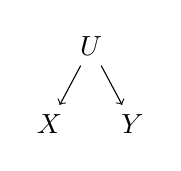
\begin{tikzpicture}[comment/.style={rectangle, text centered}]
			\centering
			\node (u) {$U$};
			\node (X) [below=0.5 of u, xshift=-1.5em] {$X$};
			%\node (Z) [left =1.5em of D] {$Z$};
			\node (Y) [below=0.5 of u, xshift=1.5em] {$Y$};
			
			\draw [->] (u) -- node [auto]{}  (X);
			\draw [->] (u) -- node [auto]{}  (Y);
			%\draw [->] (D) -- node [auto]{}  (Y);
			%\draw [->] (Z) -- node [auto]{}  (D);
			%\draw[<->, >=latex', shorten >=2pt, shorten <=2pt, bend right=30, thick, color=red] 
			%(Z.south) to node[auto, swap] {exclusion restriction}(Y.south);
			%\node  [comment, below = 0.08 of D] (1) {\Large\color{red}$\times$};
		\end{tikzpicture}
	\end{figure}
	
	
	\begin{itemize}
		\item $X$ (Chocolate Consumption) is associated (correlated) with $Y$ (Number of Nobel Laureates) 
		\vspace{0.2cm}
		\item Even if $X$ has no causal effect on $Y$
		\vspace{0.2cm}
		\item Since confounding factor $U$ (GDP) can result in the co-movement between $X$ and $Y$
		
		
		
	\end{itemize}
\end{frame}




\begin{frame}{Concluding Remarks of This Course}
\begin{itemize}
\item Many existing studies can only get \textbf{correlation} not \textbf{causality}
\vspace{0.2cm}
\item The estimated "causal effects" might confound with \textbf{selection bias} and the effects of other factors
\vspace{0.2cm}
\item Once you can estimate causal effect convincingly
\vspace{0.2cm}
\item Your finding will improve our understanding of human behaviors and society
\end{itemize}
\end{frame}





\begin{frame}{Teaching Evaluation}
\begin{itemize}
\item Please fill out a teaching evaluation of this course
\vspace{0.2cm}
\item Your feedbacks will help me improve this course
\end{itemize}
\end{frame}






\end{document} 
